% Intended LaTeX compiler: pdflatex
\documentclass[10pt,article]{article}
\usepackage[utf8]{inputenc}
\usepackage[T1]{fontenc}
\usepackage{graphicx}
\usepackage{grffile}
\usepackage{longtable}
\usepackage{wrapfig}
\usepackage{rotating}
\usepackage[normalem]{ulem}
\usepackage{amsmath}
\usepackage{textcomp}
\usepackage{amssymb}
\usepackage{capt-of}
\usepackage{hyperref}
\usepackage{titling} \posttitle{\par\end{center}} \setlength{\droptitle}{-30pt} \usepackage{multicol} \setlength{\columnsep}{1cm} \usepackage[T1]{fontenc} \usepackage[utf8]{inputenc} \renewcommand{\contentsname}{Table of Contents / Agenda} \usepackage[letterpaper,left=1in,right=1in,top=0.7in,bottom=1in,headheight=23pt,includehead,includefoot,heightrounded]{geometry} \usepackage{fancyhdr} \pagestyle{fancy} \fancyhf{} \cfoot{\thepage} \usepackage{mathpazo} \usepackage[scaled=0.85]{helvet} \usepackage{courier} \usepackage[onehalfspacing]{setspace} \usepackage[framemethod=default]{mdframed} \usepackage{wrapfig} \usepackage{booktabs} \usepackage[outputdir=Lectures]{minted}
\setcounter{secnumdepth}{3}
\date{\vspace{-6ex}}
\title{Class 1: Introduction}
\hypersetup{
 pdfauthor={},
 pdftitle={Class 1: Introduction},
 pdfkeywords={},
 pdfsubject={Fall 2018 Org-Coursepack School specific teaching materials},
 pdfcreator={Emacs 26.1 (Org mode 9.1.14)}, 
 pdflang={English}}
\begin{document}

\maketitle
\lhead{ ORG 0000 \\ Joon H. Ro \& Jae-Eun Namkoong } 
\rhead{ Class 1 \\ 2018-08-28 Tue} 
\thispagestyle{fancy}

\setcounter{tocdepth}{1}
\tableofcontents
\vspace{6ex}

\section{Introduction to Org-Coursepack}
\label{sec:org9bff693}
The Org-Coursepack provides a template for developing and managing teaching
materials using \href{https://orgmode.org/manual/Export-settings.html}{Org mode}, a major mode in \href{https://www.gnu.org/software/emacs/manual/html\_node/emacs/Specifying-File-Variables.html\#Specifying-File-Variables}{GNU Emacs}.
\subsection{Advantages for Instructors}
\label{sec:orgbf83241}
\begin{itemize}
\item First, Org mode and modular design allow for more effective and efficient
content creation.
\begin{itemize}
\item Content updates get propagated across courses, semesters, and sections,
minimizing the potential for inconsistencies
\item Minimizes redundancy when sharing content across courses, semesters, and
sections
\end{itemize}
\end{itemize}

\begin{itemize}
\item Second, instructors can enjoy the benefits of having a flexible export system and an output-specific export option.
\begin{itemize}
\item Consistent content across multiple output formats
\begin{itemize}
\item Slides (e.g., via reveal.js or Beamer backends)
\item Handouts (e.g., via the \LaTeX{} or reStructuredText backends)
\end{itemize}
\item Selective formatting and presentation of components depending on output
format
\end{itemize}
\item Third, the template contains a) utility functions written in Emacs Lisp, b)
shortcuts to Org mode functions, and c) pre-built tree structures, which
allow automation of many tasks including:
\begin{itemize}
\item Automatic class numbering
\item Automatic creation of key content including (but not limited to)
\begin{itemize}
\item course schedule for syllabi;
\item agenda of lecture materials; and
\item exam keys.
\end{itemize}
\end{itemize}
\end{itemize}
\subsection{Advantages for Students}
\label{sec:orgd1ed15e}
\begin{itemize}
\item Consistent, properly-formatted, and strategically presented course materials add to student engagement
\item Availability of materials that are easier to digest and review outside the classroom
\end{itemize}
\subsection{Requirements}
\label{sec:org3808cae}
\begin{itemize}
\item Org-Coursepack is a tool based on \href{https://orgmode.org/manual/Export-settings.html}{Org mode}, a major mode in \href{https://www.gnu.org/software/emacs/manual/html\_node/emacs/Specifying-File-Variables.html\#Specifying-File-Variables}{GNU Emacs}. It
does not, however, require extensive previous experience with either, unless
the user wants to make changes to pre-built scripts. The basic level of
knowledge needed is:
\begin{description}
\item[{Emacs}] Basic knowledge of text editing using Emacs
\item[{Org mode}] Basic knowledge of Org mode markup syntax. Org mode uses a
straightforward markup language similar to Markdown and
reStructuredText, thus it will be easy to learn for any user
who is familiar with other markup languages.
\end{description}
\end{itemize}
\section{Quickstart Guide}
\label{sec:org68b5d44}
In this quickstart guide, we will guide you through how to create your course
with \texttt{Org-Coursepack} with step-by-step examples. We focus on syllabi and lectures, 
as they tend to make up for the majority of the course content, and other parts such as 
assignments and exams can be created similarly.
\subsection{Copy and rename \texttt{Template} course}
\label{sec:orgbc82294}
We use \texttt{/} as the root path of Org-Coursepack throughout this quickstart
guide. Make a copy of the \texttt{Template} directory inside \texttt{/Courses} folder and
rename the folder and \texttt{template.org} inside the folder to your course name. We
call this \texttt{Org-Coursepack-Quickstart-Guide} in this tutorial:

\begin{center}
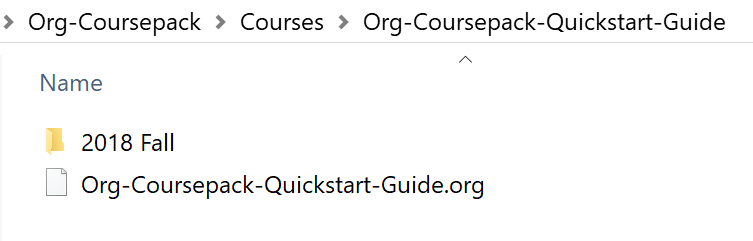
\includegraphics[width=8cm]{../../../Assets/Images/Org-Teaching/Quickstart_Course-renamed.png}
\end{center}

Your specific course for a semester will reside inside \texttt{Semester} folder. We
assume that you are preparing a course for the fall 2018 semester -- let's
rename the folder and \texttt{Semestor.org} inside the folder to \texttt{2018 Fall} and
\texttt{2018 Fall.org}, respectively. From this semester Org file you will be
exporting your actual course content.

\begin{center}
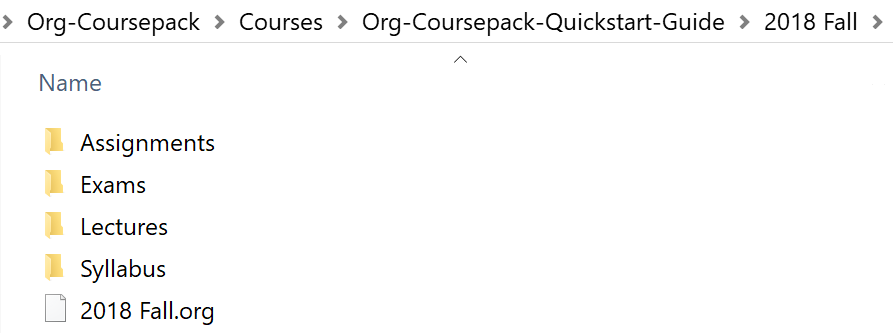
\includegraphics[width=10cm]{../../../Assets/Images/Org-Teaching/Quickstart_Semester-renamed.png}
\end{center}
\subsection{Set local variables permission in semester Org file}
\label{sec:orgc210200}
Visit (i.e., open) \texttt{2018 Fall.org}. First time you visit this file, it will 
show you the following warning about local variables:

\begin{minted}[]{common-lisp}
  The local variables list in 201 Fall.org
  contains values that may not be safe (*), and variables that are risky (**)
\end{minted}

These variables have time-format settings, as well as
\texttt{org-confirm-elisp-link-function: nil}, which allows you to click on links
(mainly for exporting) without being asked to confirm. You can type \texttt{!} to set
them permanently for your convenience.

Then you will see that the file is open and it has a template to construct a
course for this semester:

\begin{center}
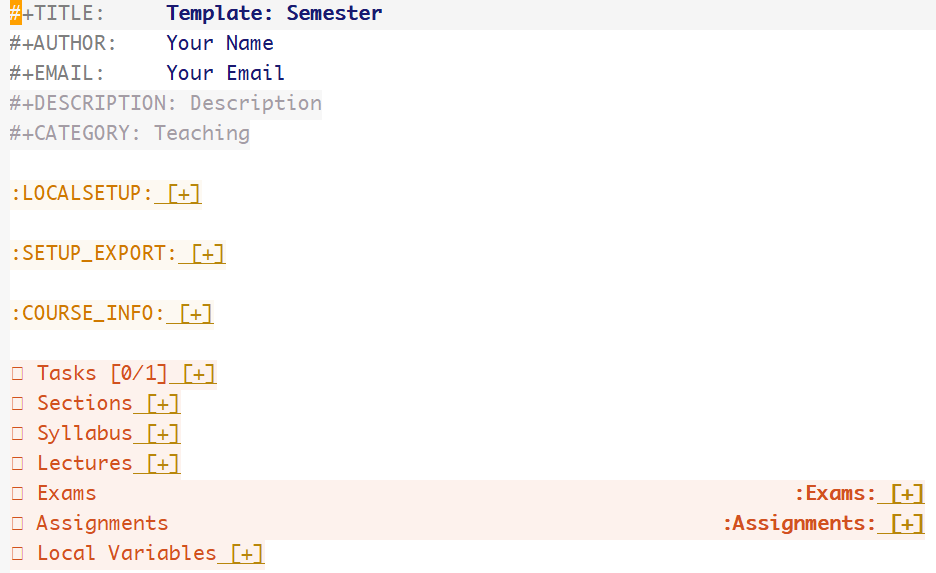
\includegraphics[height=7cm]{../../../Assets/Images/Org-Teaching/Quickstart_Semester-Org-File.png}
\end{center}

You can freely move around with movement keys. Drawers (e.g., \texttt{:LOCALSETUP:})
and subtrees (e.g., \texttt{* Sections}) under the cursor can be expanded and
collapsed by pressing \texttt{Tab} key:

\begin{center}
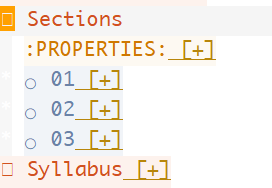
\includegraphics[height=2cm]{../../../Assets/Images/Org-Teaching/Quickstart_Org-Expand.png}
\end{center}

\subsection{Rename paths to semester and course Org files for \texttt{\#+INCLUDE} statements}
\label{sec:org19895a3}
The semester Org file has many \texttt{\#+INCLUDE} statements which refer to the
semester Org itself and the course Org file. We should rename paths to these
files so \texttt{\#+INCLUDE} statements work property.

First, you should replace all occurrences of \texttt{./Semester.org::} with the name
of the current semester Org file, \texttt{./2018 Fall.org::}. This can be achieved in
Emacs by pressing \texttt{M-\%} (\texttt{Alt+Shift+5}, or via \texttt{Edit} -> \texttt{Replace} -> \texttt{Replace
String} menu), and inputting \texttt{./Semester.org::<Enter>} followed by \texttt{./2018
Fall.org::<Enter>}, and pressing \texttt{!} (replace all). Emacs will let you know
how many replaces it has done. The query replace will look like the following:

\begin{verbatim}
  Query replace ./Semester.org with: ./2018 Fall.org
\end{verbatim}

So all \texttt{./Semester.org::} are replaced by \texttt{./2018 Fall.org::}:

\begin{multicols}{2}
\begin{center}
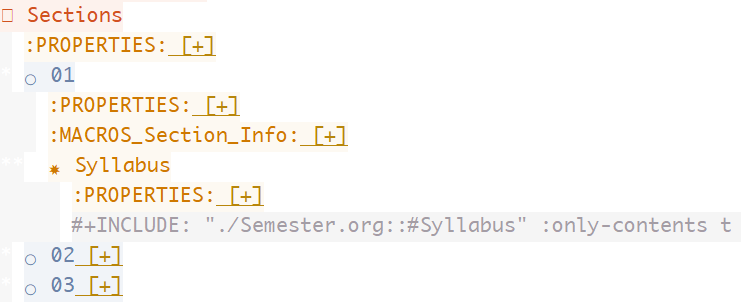
\includegraphics[height=3cm]{../../../Assets/Images/Org-Teaching/Quickstart_Semester-Rename-Semester-Before.png}
\end{center}

\begin{center}
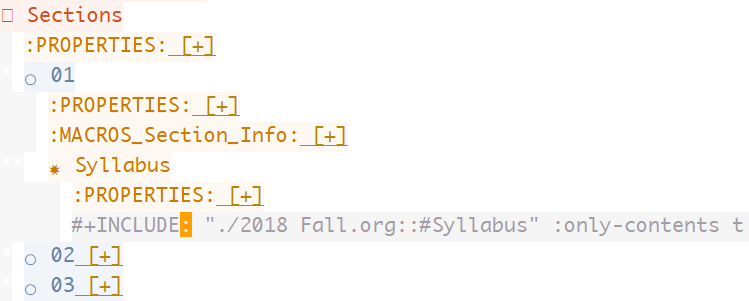
\includegraphics[height=3cm]{../../../Assets/Images/Org-Teaching/Quickstart_Semester-Rename-Semester-After.png}
\end{center}
\end{multicols}


Then, replace \texttt{../Template.org::} with the name of your course Org file in the
same way. In this quickstart guide,

\begin{verbatim}
  Query replace ../Template.org:: with: ../Org-Coursepack-Quickstart-Guide.org::
\end{verbatim}

So all \texttt{../Template.org::} are replaced by \texttt{../Org-Coursepack-Quickstart-Guide.org::}:

\begin{multicols}{2}
\begin{center}
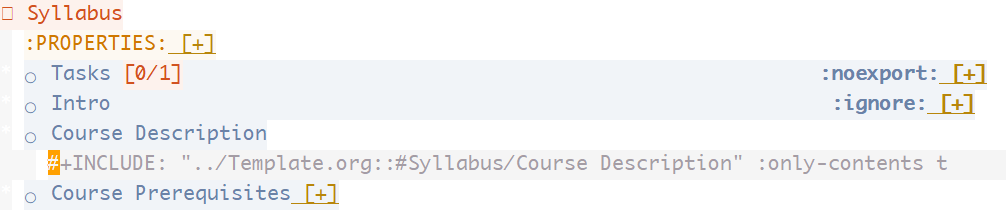
\includegraphics[height=3cm]{../../../Assets/Images/Org-Teaching/Quickstart_Semester-Rename-Course-Before.png}
\end{center}

\begin{center}
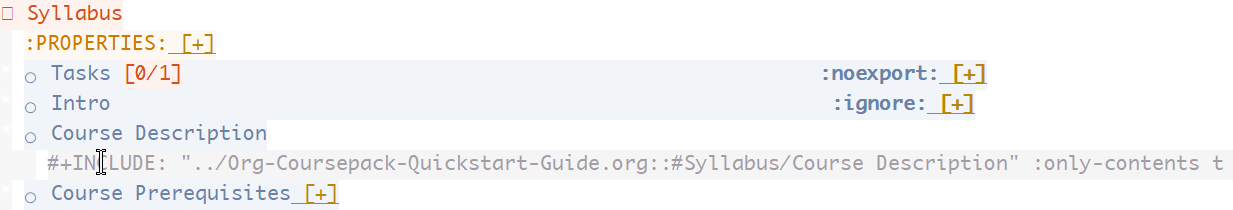
\includegraphics[height=3cm]{../../../Assets/Images/Org-Teaching/Quickstart_Semester-Rename-Course-After.png}
\end{center}
\end{multicols}
\subsection{Inputting course information}
\label{sec:orge6a2158}
The first several lines of the semester Org file (\texttt{2018 Fall.org}) contain
multiple course information values, such as the \texttt{\#+TITLE:} and
\texttt{\#+DESCRIPTION:}. Also, You can press \texttt{Tab} key while your cursor is on
\texttt{:COURSE\_INFO:} to expand the drawer, revealing other information such as
\texttt{COURSE} and \texttt{SEMESTER}. They currently have filler values:

\begin{center}
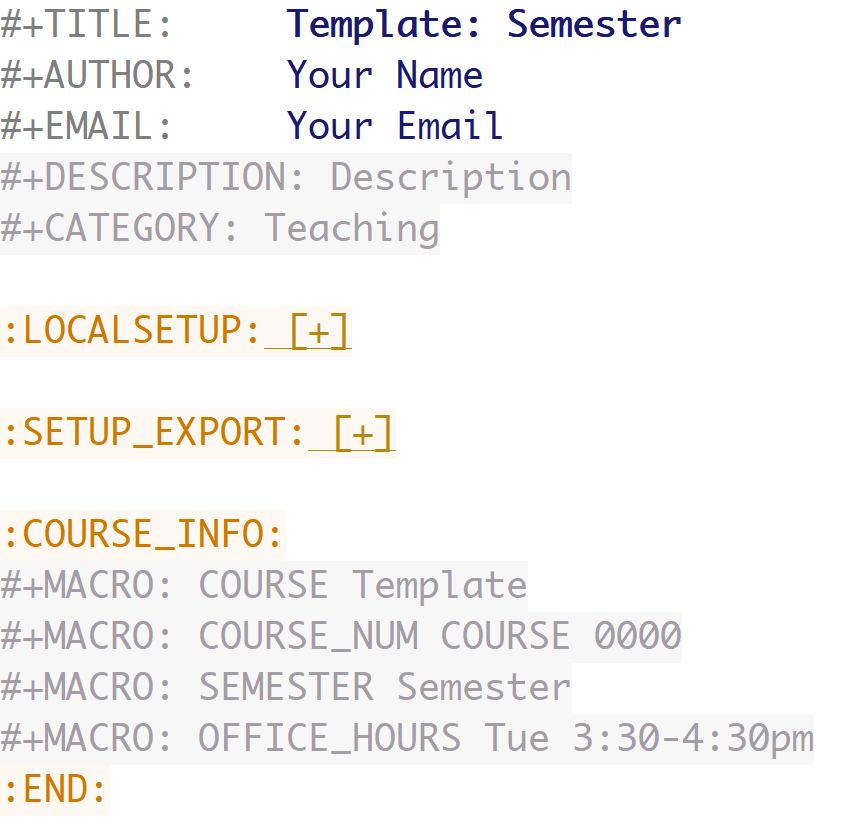
\includegraphics[height=6cm]{../../../Assets/Images/Org-Teaching/Quickstart_Semester-Course-Info.png}
\end{center}

You can fill them with relevant information:

\begin{center}
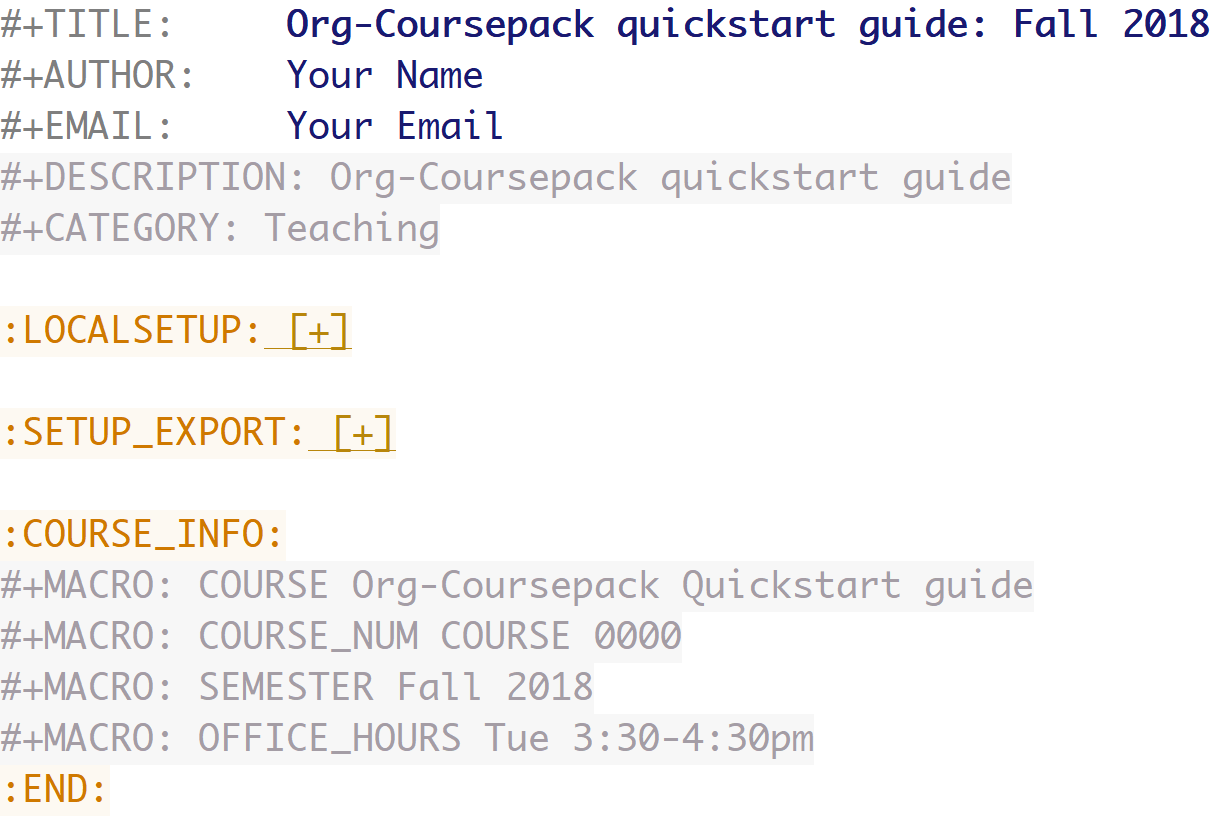
\includegraphics[height=6cm]{../../../Assets/Images/Org-Teaching/Quickstart_Semester-Course-Info-Edited.png}
\end{center}
\subsection{Preparing your syllabus}
\label{sec:org8230666}
\subsubsection{Exporting syllabus}
\label{sec:orgb6728f7}
Let's prepare your syllabus. First, let's see how the output looks like by
exporting the current syllabus. Navigate to \texttt{* Sections/01/Syllabus} subtree.
You can expand and collapse subtrees by pressing \texttt{Tab} key. Expand
\texttt{:PROPERTIES:} of the \texttt{* Sections/01/Syllabus} subtree by pressing \texttt{Tab}. It
has built-in clickable links for \LaTeX{} export \texttt{LaTeX (Custom Time Format)}.
Clicking on this link (see the screenshot below) will export the syllabus for
the section 1 to the \texttt{Syllabus} sub-directory.

\begin{center}
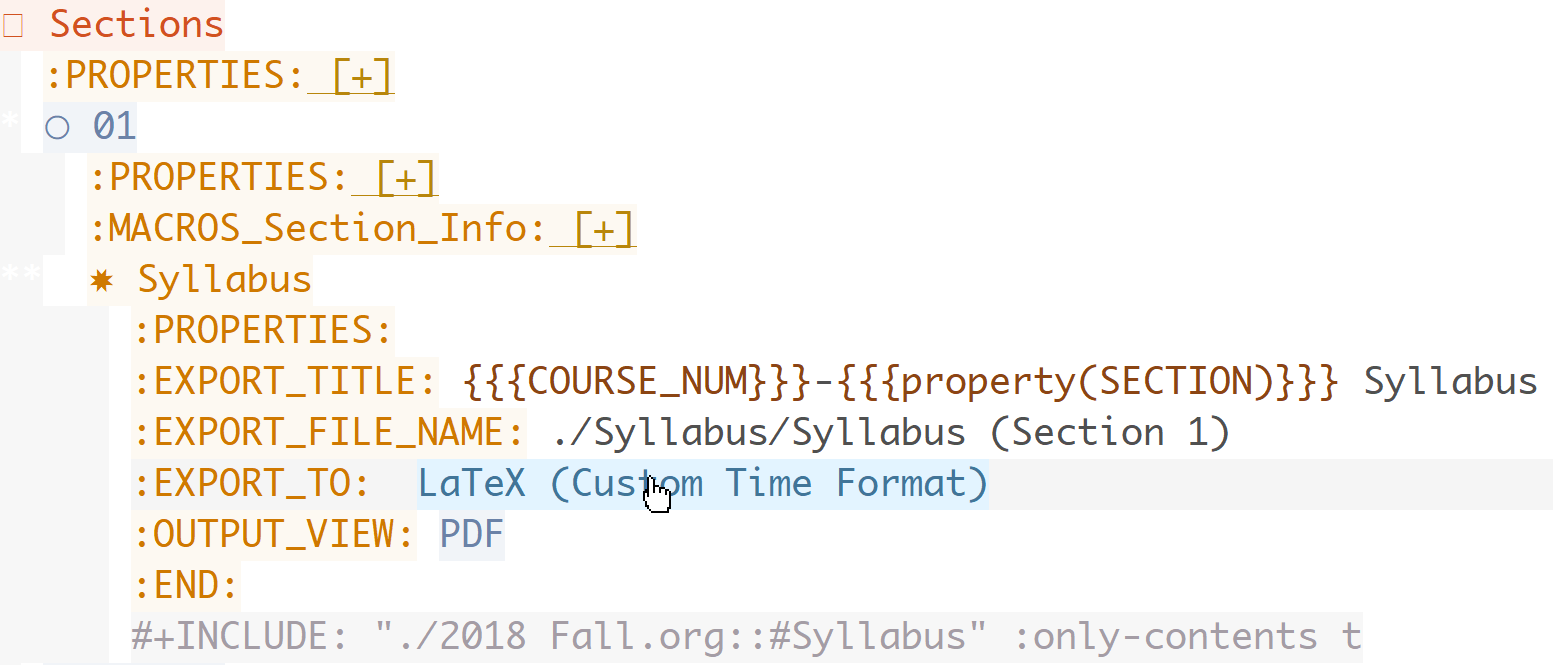
\includegraphics[width=10cm]{../../../Assets/Images/Org-Teaching/Quickstart_Syllabus-Export-Link.png}
\end{center}

Once export is finished, clicking on the \texttt{PDF} link will open the exported
output in your default pdf viewer:

\begin{center}
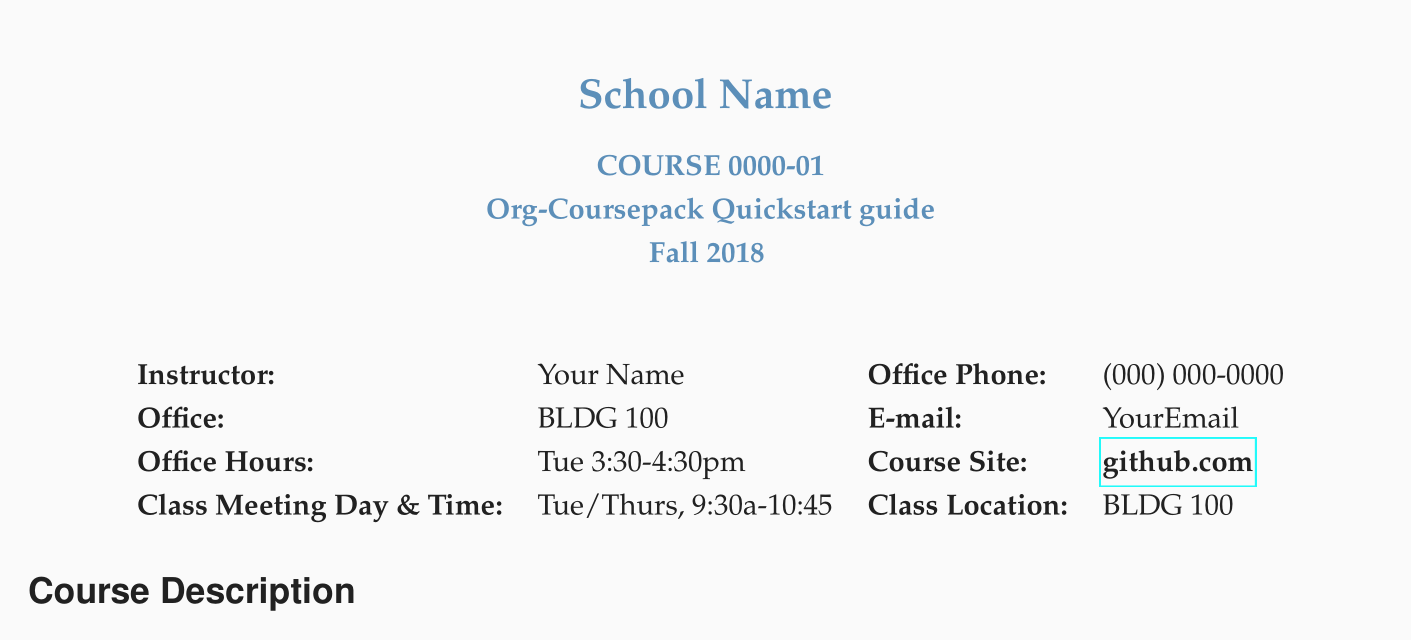
\includegraphics[width=10cm]{../../../Assets/Images/Org-Teaching/Quickstart_Exported-Syllabus-Course-Info.png}
\end{center}

 As you can see, it included the content
from \texttt{* Syllabus} subtree, but it used section-specific information from
\texttt{:PROPERTIES:} of the section subtree, as shown below.

\begin{center}
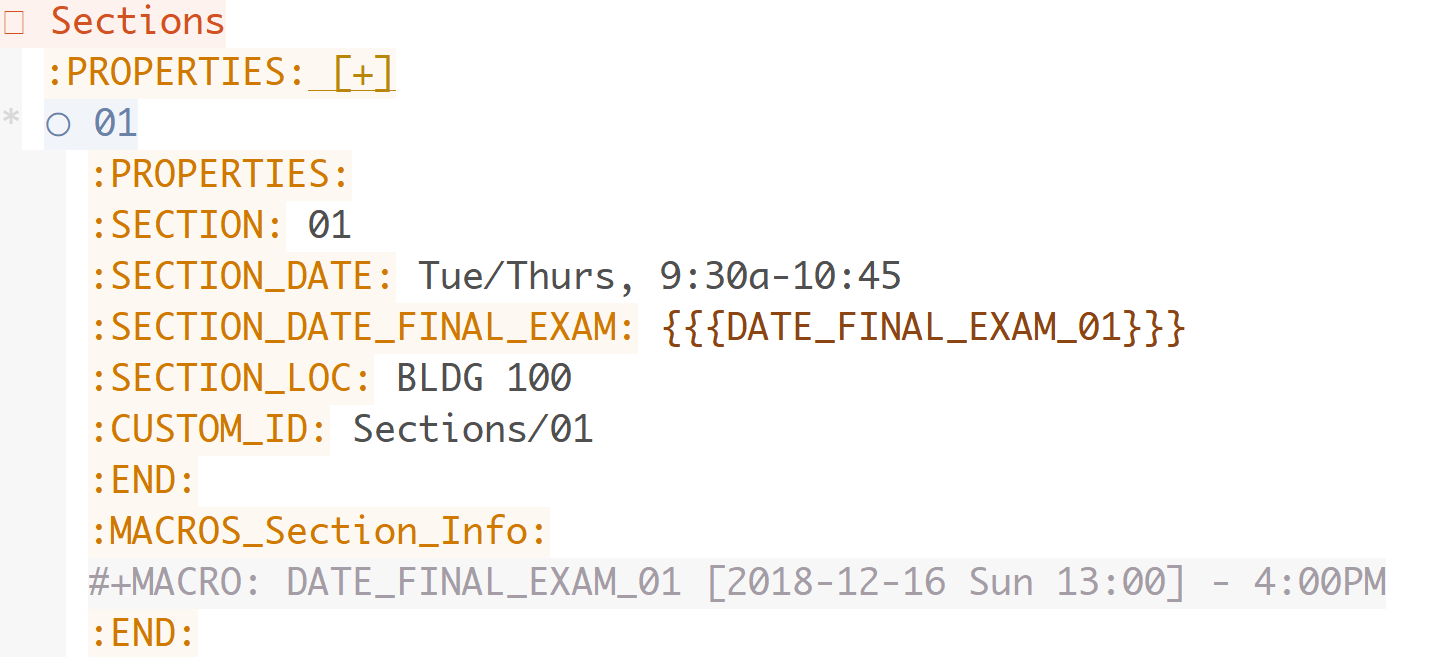
\includegraphics[width=10cm]{../../../Assets/Images/Org-Teaching/Quickstart_Section-Information-Properties.png}
\end{center}
\subsubsection{Editing syllabus content}
\label{sec:org946ac97}
While the syllabus will be exported from this semester Org file (\texttt{2018
Fall.org}), any course-specific content common across semesters, such as the
course description, are stored in the course Org file
(\texttt{Org-Coursepack-Quickstart-Guide.org}).

Let's modify the course description. Navigate to \texttt{* Syllabus/Course
Description}. When you expand \texttt{Course Description} subtree (see the screenshot
below), you will see that it just includes the content from the course Org
file (\texttt{../Org-Coursepack-Quickstart-Guide.org}). Hence we are assuming that
you will be using the common course description across semesters, but you can
organize your content flexibility with \texttt{Org-Coursepack}, so you can just add
semester-specific description here. You can even mix and match the two
approaches. For example, you can include the common part and then write
semester-specific part below the \texttt{\#+INCLUDE} statement.

\begin{center}
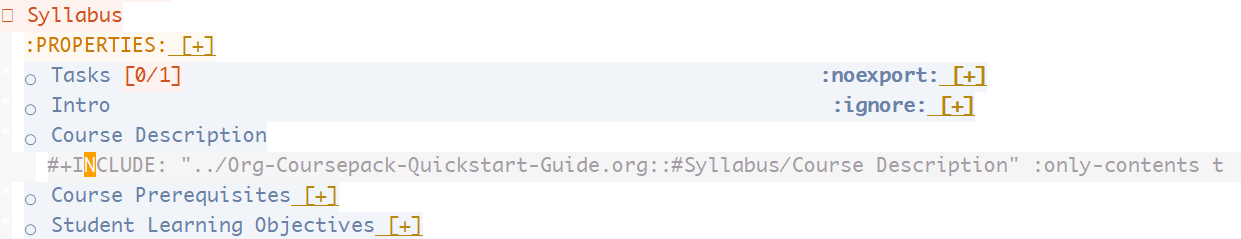
\includegraphics[height=3cm]{../../../Assets/Images/Org-Teaching/Quickstart_Syllabus-Course-Description.png}
\end{center}

While the cursor is on the \texttt{\#+INCLUDE} statement (see the screenshot above),
you can press \texttt{C-c '} (\texttt{CTRL+C} followed by \texttt{'}) to visit the file
included. You can modify the content there so it reflects the description of
your course. We add the following content there:

\begin{center}
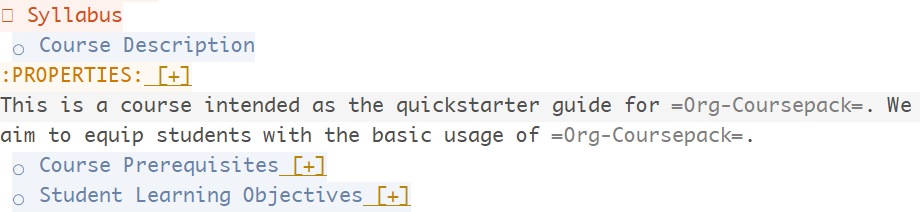
\includegraphics[height=3cm]{../../../Assets/Images/Org-Teaching/Quickstart_Syllabus-Course-Description-Content-Edited.png}
\end{center}

Now if you again click on the \LaTeX{} export button in the \texttt{:PROPERTIES:} of the \texttt{Syllabus} 
tree in the semester Org file (\texttt{2018 Fall.org}), you will see that the new course description 
is reflected in the exported pdf.

\begin{center}
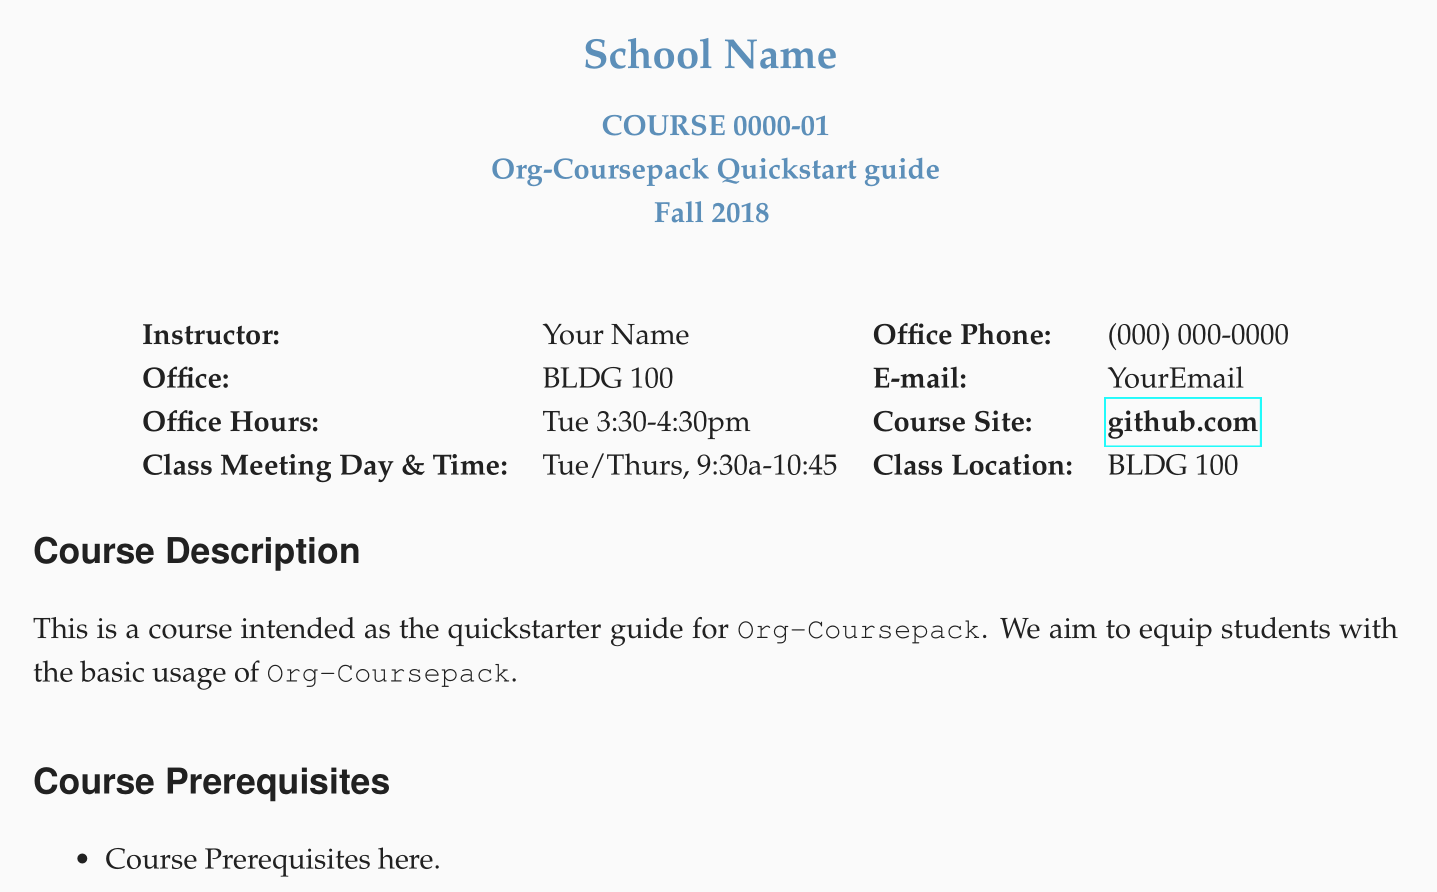
\includegraphics[height=6cm]{../../../Assets/Images/Org-Teaching/Quickstart_Syllabus-Exported-Course-Desc.png}
\end{center}

We will go to the class schedule section since users can modify other sections in the same way. 

\subsubsection{Class Schedule}
\label{sec:orgcdb4032}
\texttt{Class Schedule} section needs more explanation since \texttt{Org-Coursepack} is
designed to automatically generate the schedule of classes for your syllabus
from the list of classes. Here we will discuss only schedule-related part of
the lectures, and describe how to change actual lecture content in the next
section.

\textbf{Lecture and Assignment Dates}
Let's take a look at the \texttt{* Lectures/Lecture and Assignment Dates} subtree.

\begin{center}
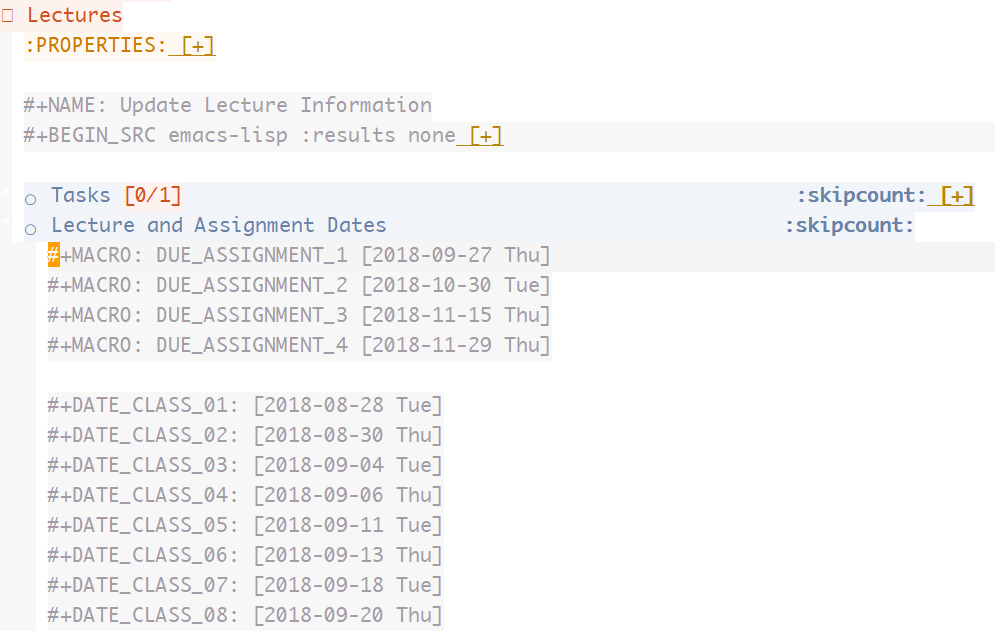
\includegraphics[height=7cm]{../../../Assets/Images/Org-Teaching/Quickstart_Lectures-Dates.png}
\end{center}

Here, currently 4 assignment due dates and 28 class dates are defined. You can
adjust these dates following your teaching schedule. These dates will be used
when we update lecture information. Org mode provides a convenient way to
adjust dates. For instance, when the cursor is on a timestamp, one can easily
adjust dates by pressing \texttt{Up} and \texttt{Down} keys with \texttt{Shift} key.

\textbf{Adding Lectures} Under the subtree \texttt{Lectures}, subtrees with \texttt{skipcount} tag
are not actual lectures, they are either subtrees which have auxiliary
information (dates, etc) or ones that are for non-lecture events such as
assignment deadlines or holidays. Currently it has only one lecture,
\texttt{Introduction}:

ㅚㅗ\begin{center}
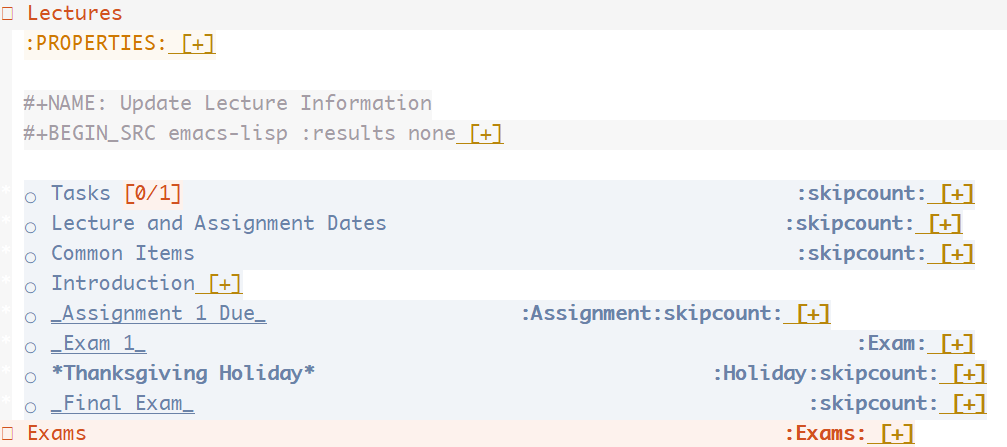
\includegraphics[height=5cm]{../../../Assets/Images/Org-Teaching/Quickstart_Lectures-Lectures.png}
\end{center}

Let's add additional two lectures by copying \& pasting the \texttt{Introduction}
subtree. Then, let's change the name of these lecture subtrees. We will simply
call them \texttt{Second Lecture} and \texttt{Third Lecture}:

\begin{center}
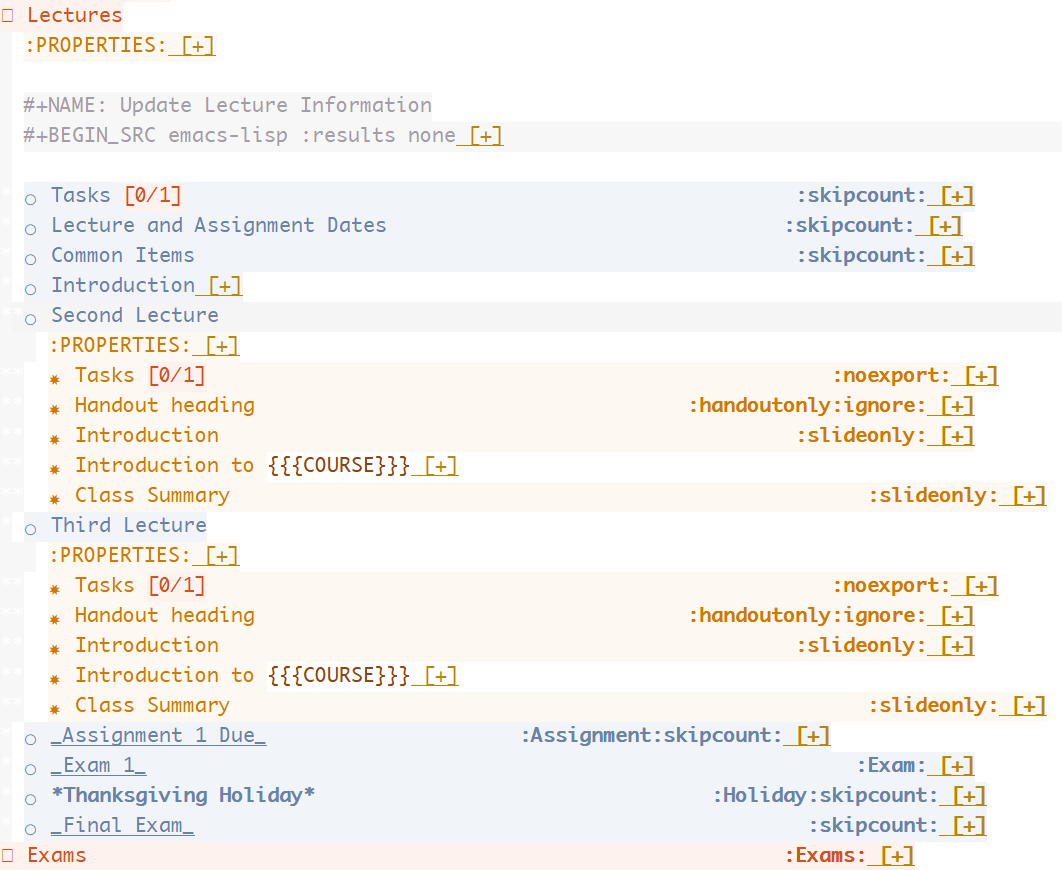
\includegraphics[height=8cm]{../../../Assets/Images/Org-Teaching/Quickstart_Lectures-Second-Lecture.png}
\end{center}

\textbf{Updating Lecture Information} When you expand \texttt{:PROPERTIES:} of the \texttt{Second
Lecture}, you will notice that it has multiple information that needs to be
updated, such as \texttt{CLASS}, \texttt{EXPORT\_FILE\_NAME}, and \texttt{DATE}. \texttt{Org-Coursepack}
provides a convenient script \texttt{Update Lecture Information} written in
Emacs-lisp which update these values as well as other elements of lectures
that depend on the schedule (e.g., agenda of the current and the previous
lectures) automatically.

Move your cursor to the script named \texttt{Update Lecture Information}, which is
located right under the \texttt{Lectures} subtree headline. You can run this script
by \texttt{C-c C-c} (\texttt{CTRL+c} and \texttt{c} while pressing \texttt{CTRL} down). 

\begin{center}
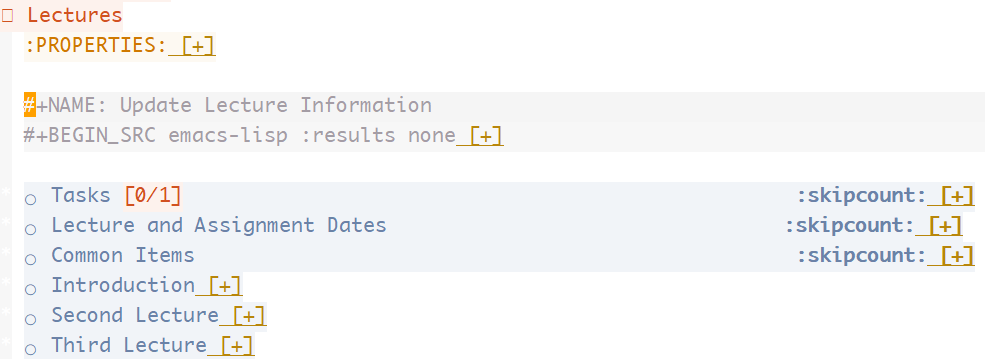
\includegraphics[height=3cm]{../../../Assets/Images/Org-Teaching/Quickstart_Lectures-Run-Script-Update-Lectures.png}
\end{center}

Emacs will ask to confirm, and you can press \texttt{y} key to do so.

\begin{center}
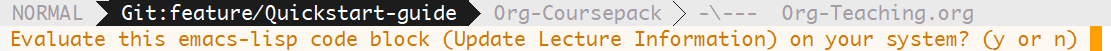
\includegraphics[width=11cm]{../../../Assets/Images/Org-Teaching/Quickstart_Lectures-Run-Script-Update-Lectures-Confirm.png}
\end{center}

Upon running the script, you will notice that the rendering of the subtrees are broken:

\begin{center}
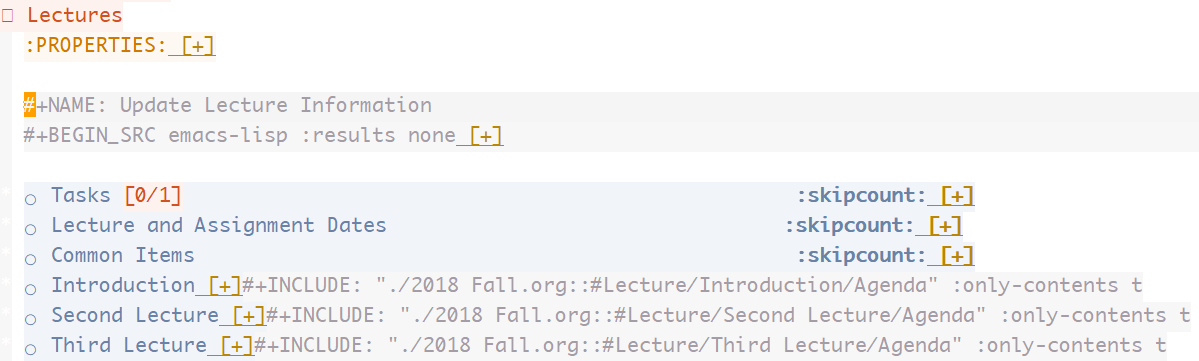
\includegraphics[height=3cm]{../../../Assets/Images/Org-Teaching/Quickstart_Lectures-Run-Script-Update-Lectures-After.png}
\end{center}

You can simple press \texttt{Shift+Tab} to collapse all the subtrees to reset the rendering.

Now let's inspect \texttt{:PROPERTIES:} for the \texttt{Second Lecture} again. Press \texttt{Tab}
key to expand \texttt{:PROPERTIES:}:

\begin{center}
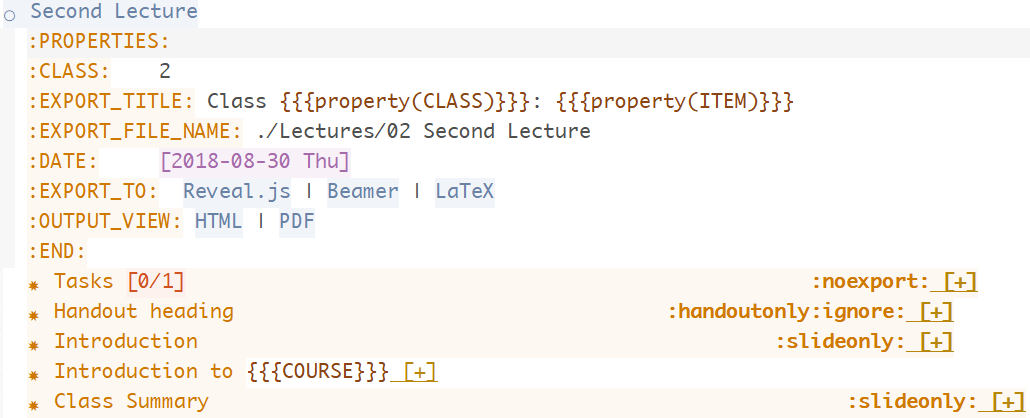
\includegraphics[height=4cm]{../../../Assets/Images/Org-Teaching/Quickstart_Lectures-Updated-Lecture-Info.png}
\end{center} 

As you can see, the script has updated information for the second (and the
third) lecture appropriately. The class number reflects the order of the
subtree. Then, the script grabs the corresponding date from the date specified
in \texttt{* Lectures/Lecture and Assignment Dates}. It also extract the name of the
lecture from the subtree headline, and then use it and the class number to
construct \texttt{EXPORT\_FILE\_NAME}. The script also does other things, which we will
describe in the next section. For non-lecture items, you can tag them with
\texttt{skipcount} tag and the script will ignore them. You can edit tags of a headline 
with \texttt{C-c q} (\texttt{CTRL+c} and \texttt{q} while pressing \texttt{CTRL} down).

\textbf{Updating Schedule} Now we are ready to update the class schedule in
Syllabus. Navigate to \texttt{* Syllabus/Class Schedule}, and then place your cursor
to the line starting with \texttt{\#+BEGIN: columnview}. If you expand the columnview, 
you will see that it has a table with previous classes. 

\begin{center}
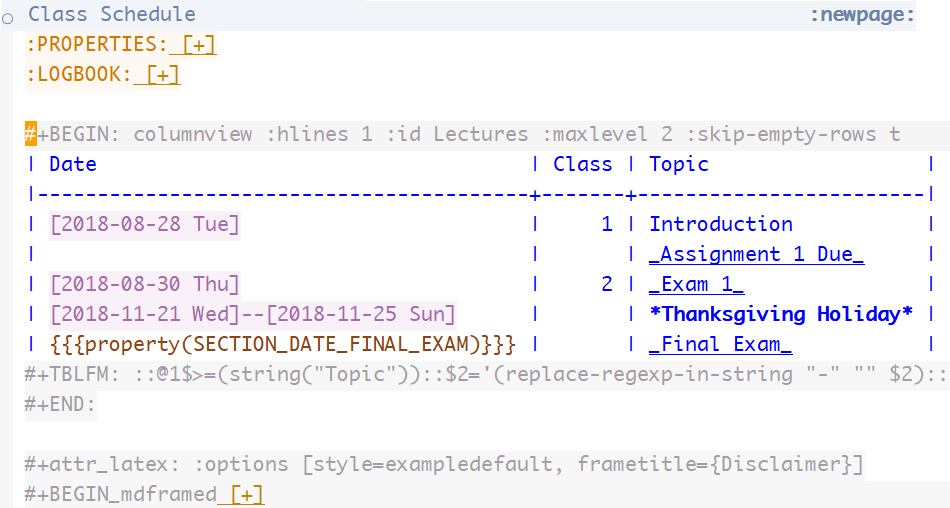
\includegraphics[height=5cm]{../../../Assets/Images/Org-Teaching/Quickstart_Syllabus-Schedule-Old.png}
\end{center}

Pressing \texttt{C-c C-c} will update the table:

\begin{center}
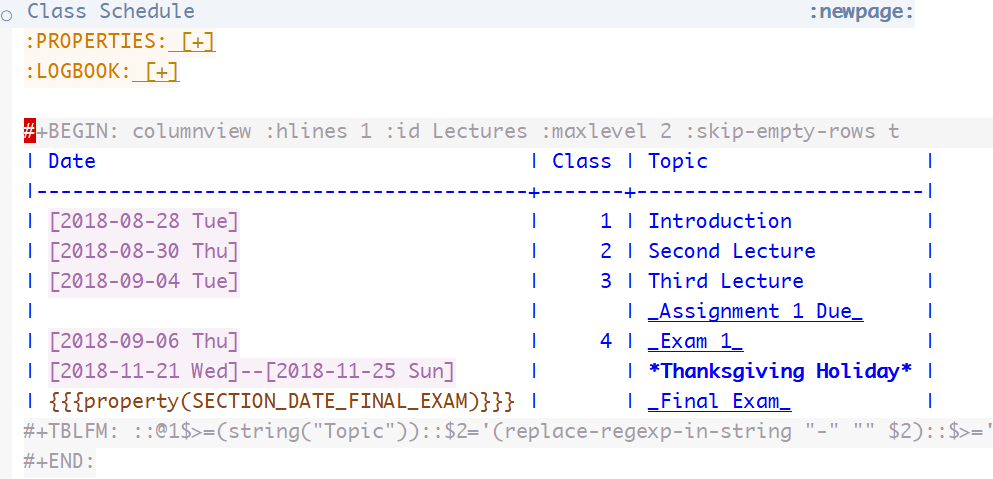
\includegraphics[height=5cm]{../../../Assets/Images/Org-Teaching/Quickstart_Syllabus-Schedule-New.png}
\end{center}

As you can see, the columnview automatically extract relevant information from
each lecture subtree in creating the table. Hence, the user can freely
re-organize lectures and change their names without worrying about updating
lecture information or class schedule manually.

Of course, the updated schedule will be reflected when the user export the syllabus for a section:

\begin{center}
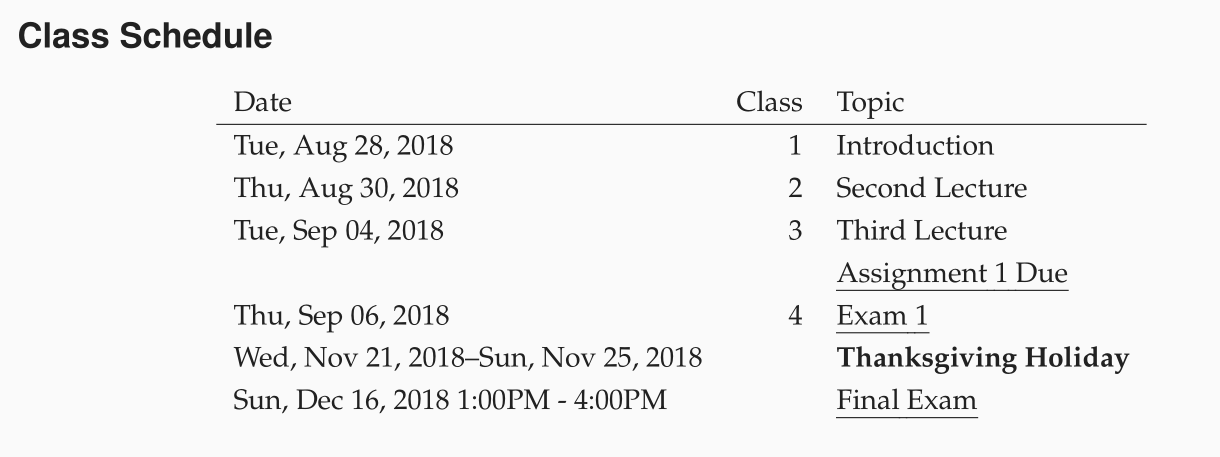
\includegraphics[height=4cm]{../../../Assets/Images/Org-Teaching/Quickstart_Syllabus-Exported-Schedule.png}
\end{center}

\subsection{Preparing your lectures}
\label{sec:org10f0594}
\subsubsection{Exporting slides and handouts}
\label{sec:orgaa96fb3}
Similar to \texttt{Syllabus} subtree under each section subtree, a lecture subtree
has built-in export links available. You can click on \texttt{reveal.js} and \texttt{LaTeX}
links to export the lecture to slide and handout formats, respectively.

\begin{center}
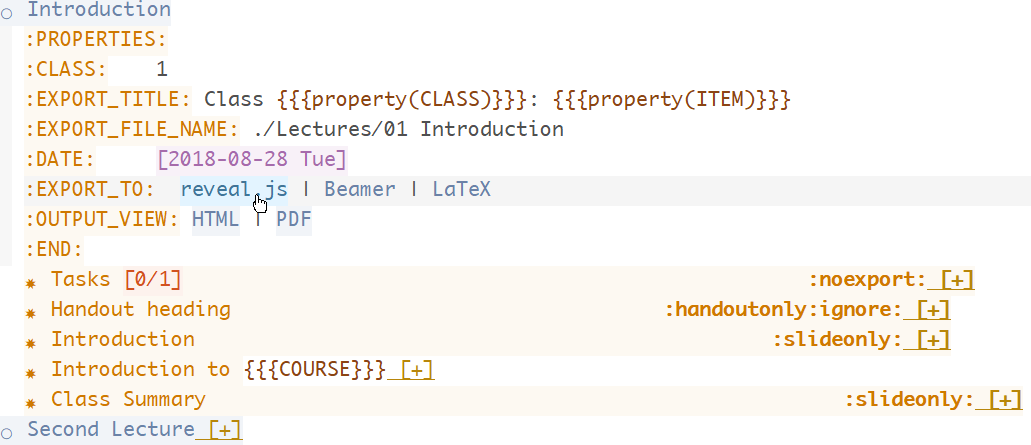
\includegraphics[height=6cm]{../../../Assets/Images/Org-Teaching/Quickstart_Lecture-Export-Link.png}
\end{center}

Let's export the lecture to both reveal.js and \LaTeX{} output formats. The files
will be exported to \texttt{Lectures} sub-directory of the semester folder. Clicking
on \texttt{HTML} and \texttt{PDF} links will open the corresponding exported file.

The following two screenshots show the exported outputs, where it is showing
the slide overview for the reveal.js slides:

\begin{center}
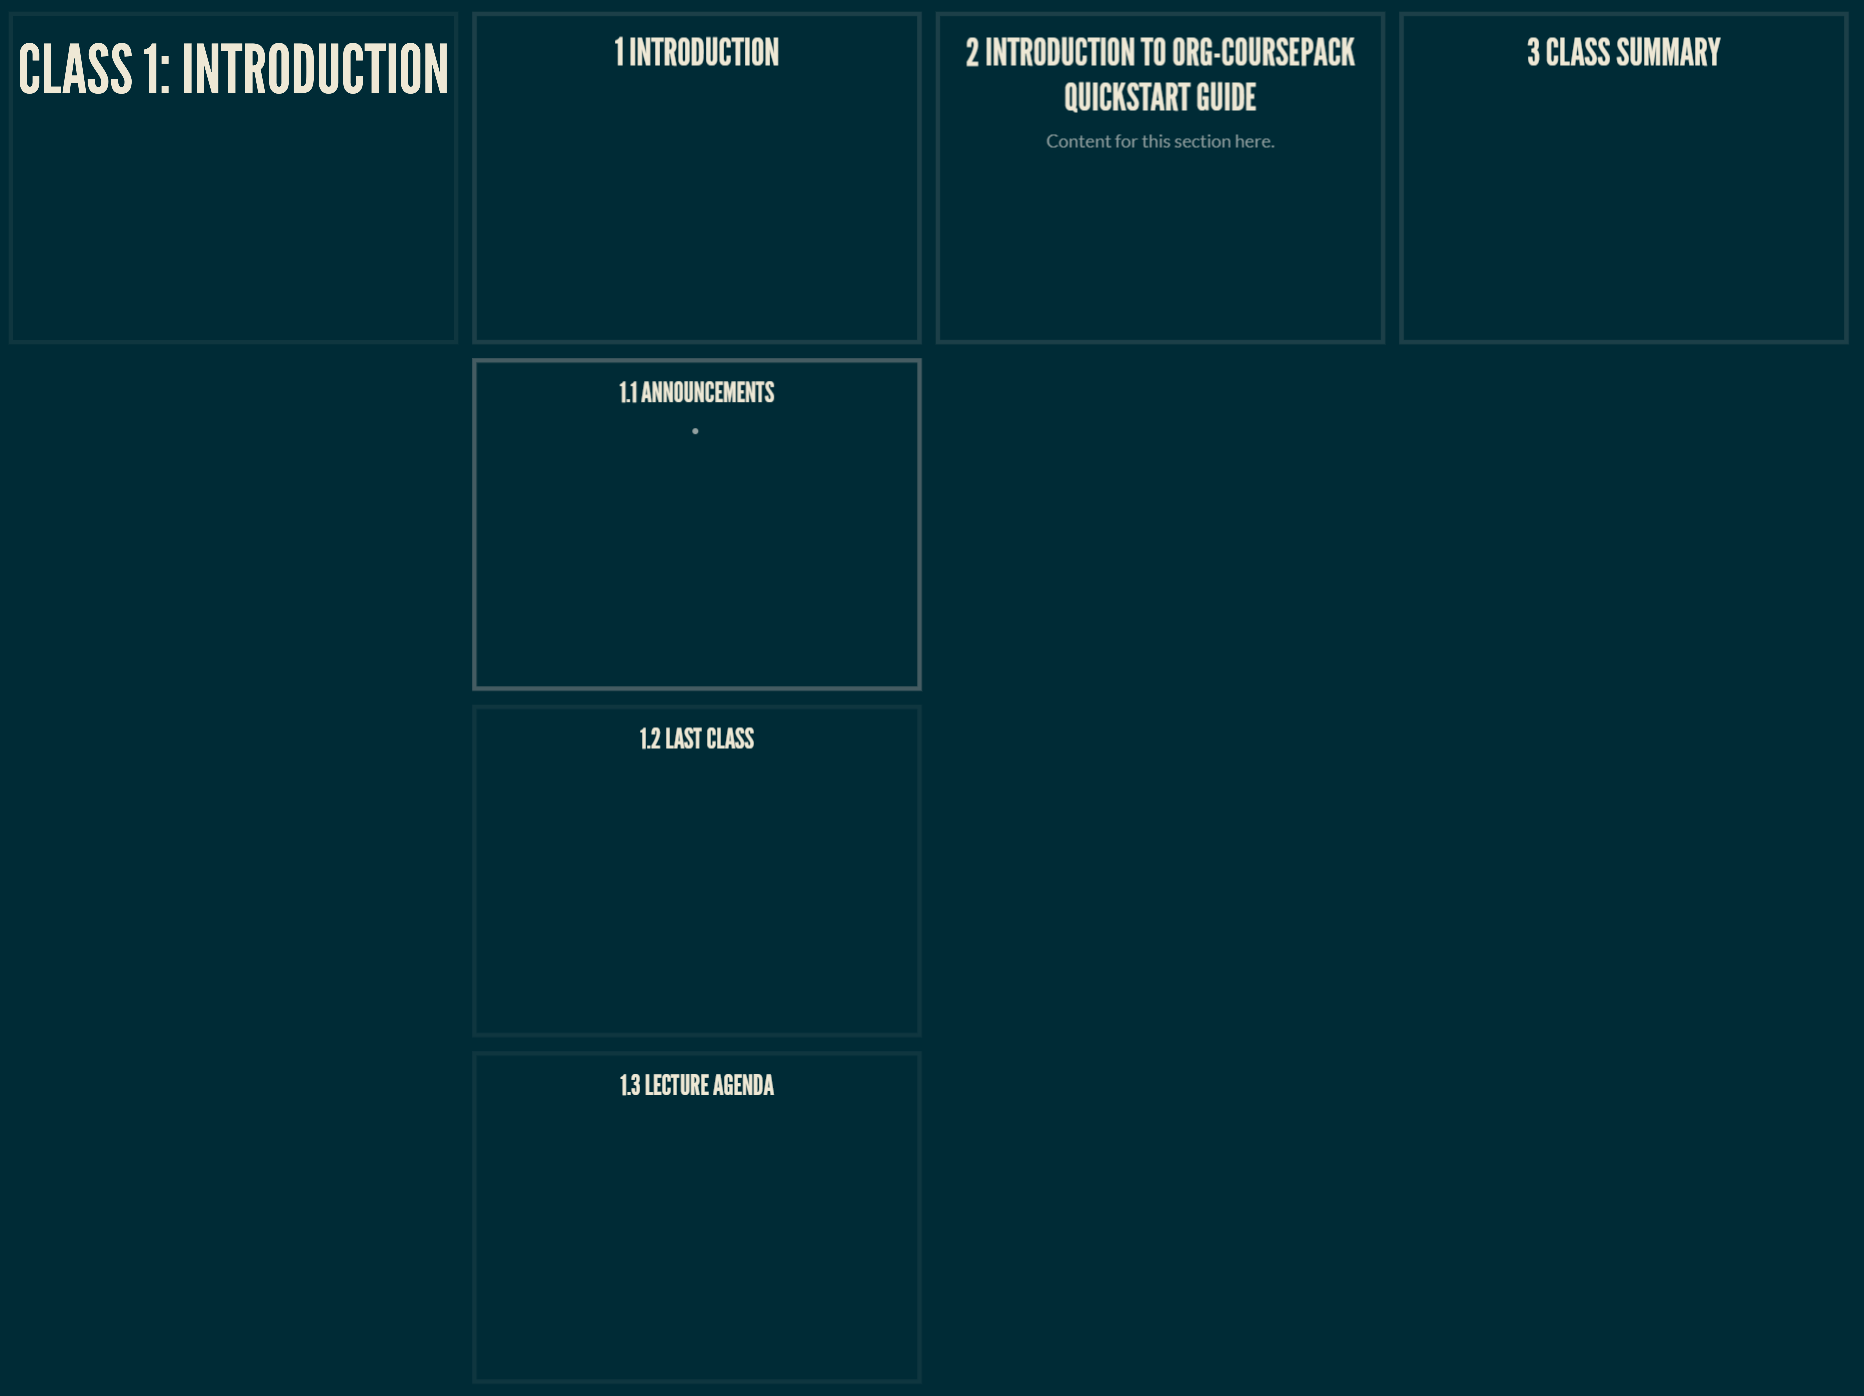
\includegraphics[height=9cm]{../../../Assets/Images/Org-Teaching/Quickstart_Lecture-Exported_reveal.png}
\end{center}

\begin{center}
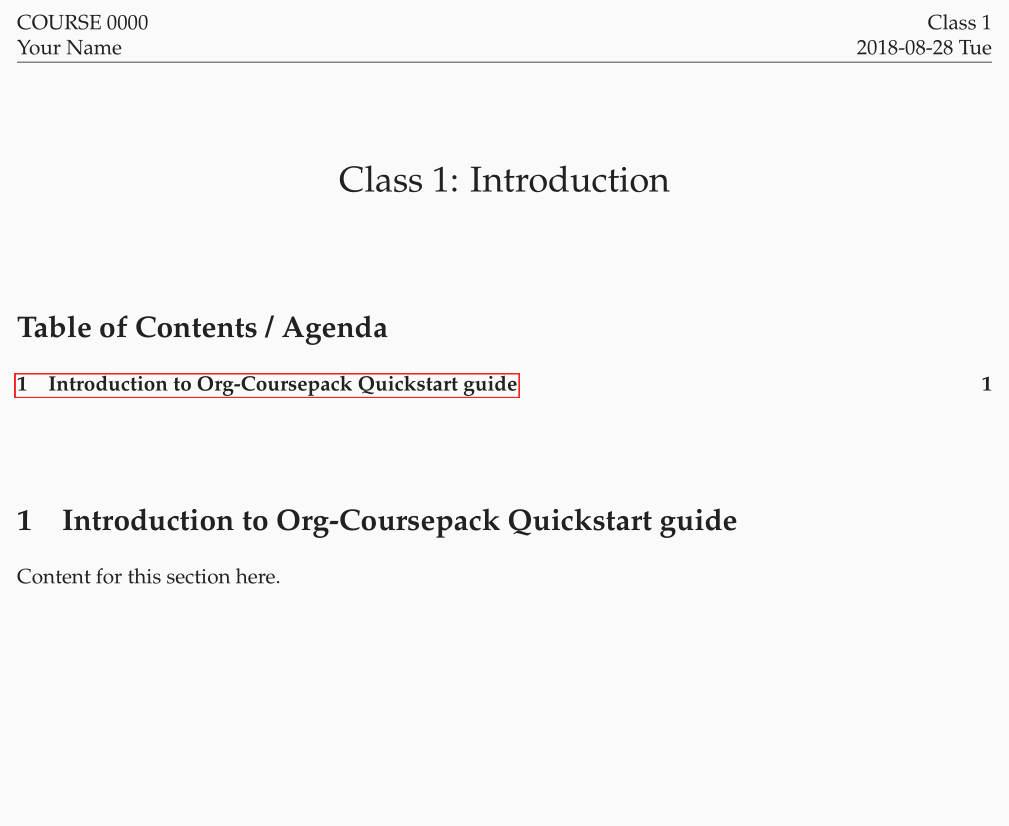
\includegraphics[height=8cm]{../../../Assets/Images/Org-Teaching/Quickstart_Lecture-Exported_LaTeX.png}
\end{center}

As you can see, the sections with \texttt{slideonly} (\texttt{handoutonly}) tag are not
exported in \LaTeX{} (reveal.js) output. You can easily specify any content you
want to show in slides (e.g., announcements) or handouts (extended explanations)
only in this way.

Also, note that the contents for \texttt{Last Class} and \texttt{Lecture Agenda} under
\texttt{Introduction} section, and \texttt{Class Summary} section are automatically written
by \texttt{Update Lecture Information} script described earlier. Hence, users can
freely edit lecture content and the order of lectures without worrying about
tediously fixing these boilerplate parts. For example, after changing the
order of lectures, the user can simply run the script and the \texttt{Last Class}
slide of each lecture will correctly point to the previous lecture in the new
order.

See \href{https://joonro.github.io/Org-Coursepack/Lectures/05\%2520Exporting\%2520Slides\%2520and\%2520Handouts.html}{Exporting Slides and Handouts} for more information about exporting
content, including setting up a key binding, which is convenient for repeated
exporting.
\subsubsection{Editing lecture content}
\label{sec:orgf7a36ca}
Let's add additional section to the lecture. Add a subtree called \texttt{New section} as the same
level as other sections (\texttt{*** New section}). 

\begin{center}
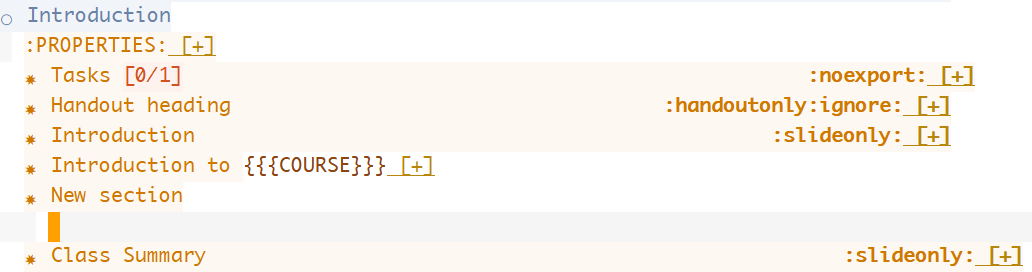
\includegraphics[height=3.5cm]{../../../Assets/Images/Org-Teaching/Quickstart_Lecture-Editing_New_Section.png}
\end{center}

You can freely use Org markup language, which is similar to other popular
markup languages such as Markdown and reStructuredText, to create your
content. The main differences are in Org mode, \texttt{*} is used to specify levels
of headings, and headings can have data associated with them in the form of
\texttt{:PROPERTIES:} and tags. In addition, navigating through a long document is 
convenient because all headings and drawers are collapsible. 

We show examples of several basic use cases here. For detailed instructions,
see \href{https://joonro.github.io/Org-Coursepack/Lectures/04\%2520Creating\%2520Content\%2520for\%2520Slides\%2520and\%2520Handouts.html}{Creating Content for Slides and Handouts} section of the documentation and
\href{https://orgmode.org/manual/index.html}{Org manual}.

\textbf{Lists} Obviously you cannot use \texttt{*} to specify a list, but otherwise Org mode
uses a typical syntax (\texttt{-} or \texttt{+} for lists, \texttt{1.} for numbered lists) for
lists. For example,

\begin{center}
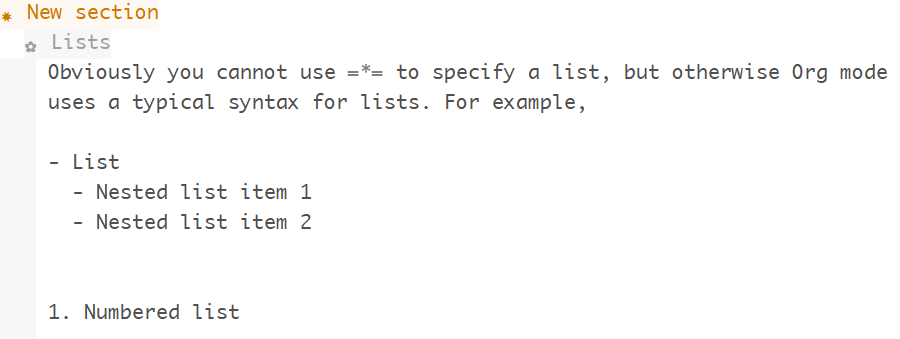
\includegraphics[height=4cm]{../../../Assets/Images/Org-Teaching/Quickstart_Lecture-Editing_Lists.png}
\end{center}

\textbf{Math} you can directly input \LaTeX{} math in Org mode. For example,

\begin{center}
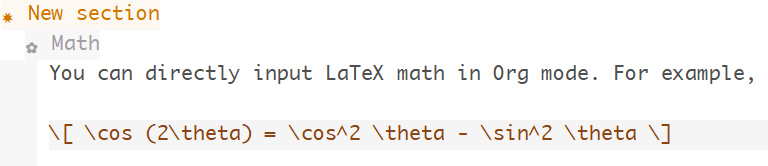
\includegraphics[height=1.8cm]{../../../Assets/Images/Org-Teaching/Quickstart_Lecture-Editing_Math.png}
\end{center}

\textbf{Slide split} in general, reveal.js will automatically create slide structure
from the lecture subtree. Sometimes, however, users might want to split a
slide into multiple slides. Users can put \texttt{\#+REVEAL: split} to split a
slide. For example,

\begin{center}
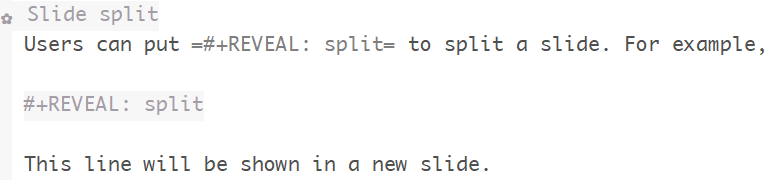
\includegraphics[height=1.8cm]{../../../Assets/Images/Org-Teaching/Quickstart_Lecture-Editing_Split.png}
\end{center}

\textbf{Fragmented contents} Fragmented contents such as lists can be easily
specified by putting \texttt{\#+ATTR\_REVEAL: :frag (appear)} before a list. For example:

\begin{center}
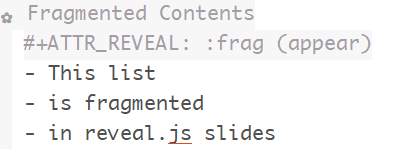
\includegraphics[height=1.8cm]{../../../Assets/Images/Org-Teaching/Quickstart_Lecture-Editing_Fragmented.png}
\end{center}

\textbf{Images} Prepending \texttt{file:} to an image file path is sufficient to include a
local image to both slide and handout. For HTML, specifying \texttt{URL} is
sufficient for an image on the web. Note that using a relative path
(\texttt{../../../Assets/Images/}) is recommended for portability. To make the image
path consistent across \LaTeX{} and HTML outputs, \texttt{<base href}"../">= is set in
\texttt{/Assets/setup\_Macros.org}.

One can also add HTML (e.g., \texttt{\#+ATTR\_HTML: :width 80\%}) and \LaTeX{}
(e.g., \texttt{\#+ATTR\_LATEX: :width 6cm}) attributes before an image link to adjust the
size of the image.

For example,

\begin{center}
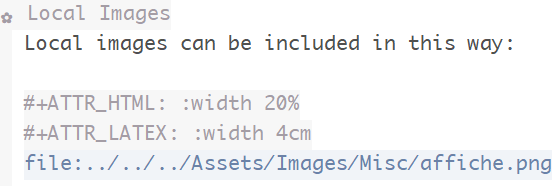
\includegraphics[height=2.5cm]{../../../Assets/Images/Org-Teaching/Quickstart_Lecture-Editing_Images.png}
\end{center}

\textbf{Hiding specific content} in addition to using \texttt{slideonly} and \texttt{handoutonly}
tags to selectively include specific subtree in export, since Org mode allows
embedding raw HTML and \LaTeX{} code, it is easy to hide specific content based
on output format. Content surrounded by \texttt{\#+LATEX: \textbackslash{}iffalse} and \texttt{\#+LATEX: \textbackslash{}fi}
will not be shown in \LaTeX{} outputs, and that surrounded by \texttt{\#+REVEAL\_HTML:
<span hidden>} and \texttt{\#+REVEAL\_HTML: </span>} will not be shown in reveal.js
output. For example, 

\begin{center}
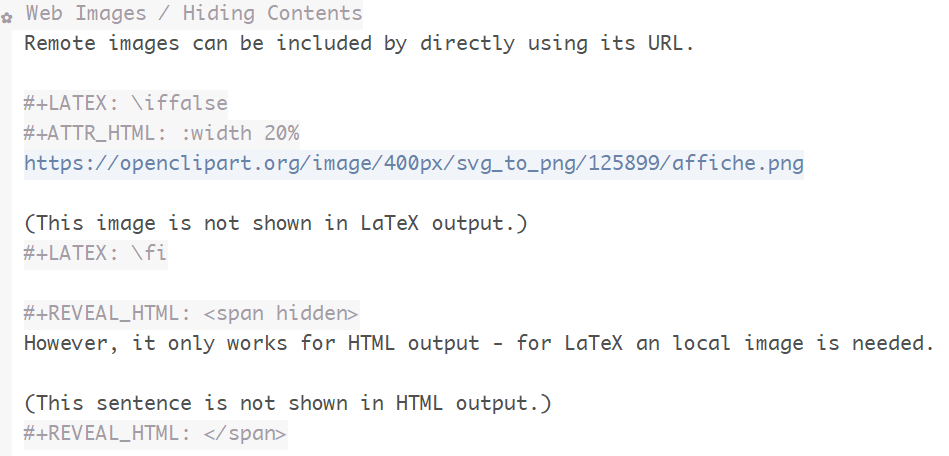
\includegraphics[height=5.5cm]{../../../Assets/Images/Org-Teaching/Quickstart_Lecture-Editing_Hiding-Contents.png}
\end{center}

The following screenshots show how they are exported:

\begin{multicols}{2}
\begin{center}
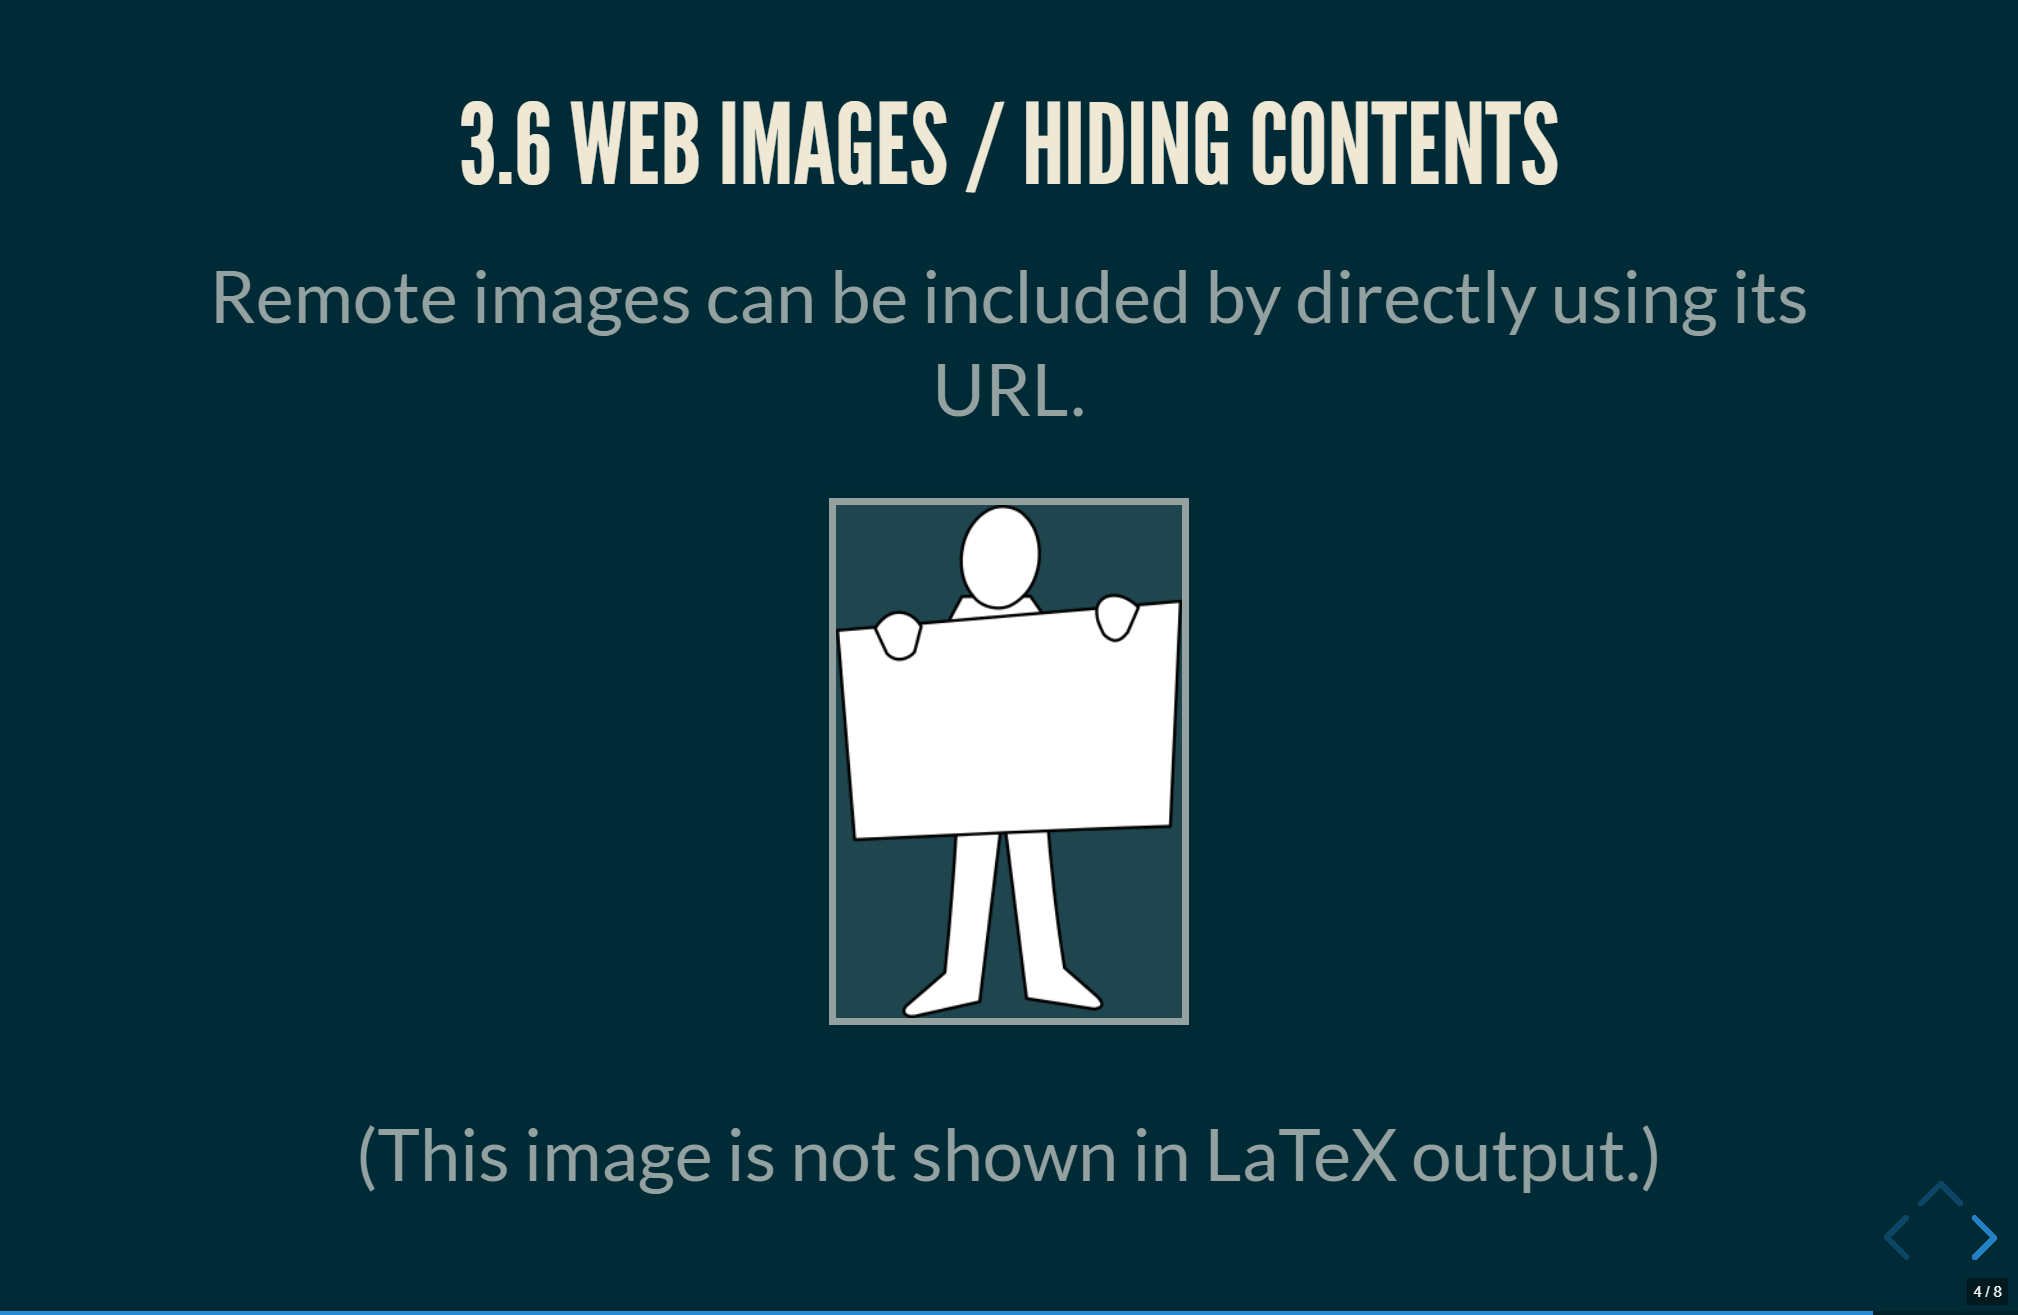
\includegraphics[width=7.5cm]{../../../Assets/Images/Org-Teaching/Quickstart_Lecture-Editing_Hiding-Contents-reveal.js.png}
\end{center}

\begin{center}
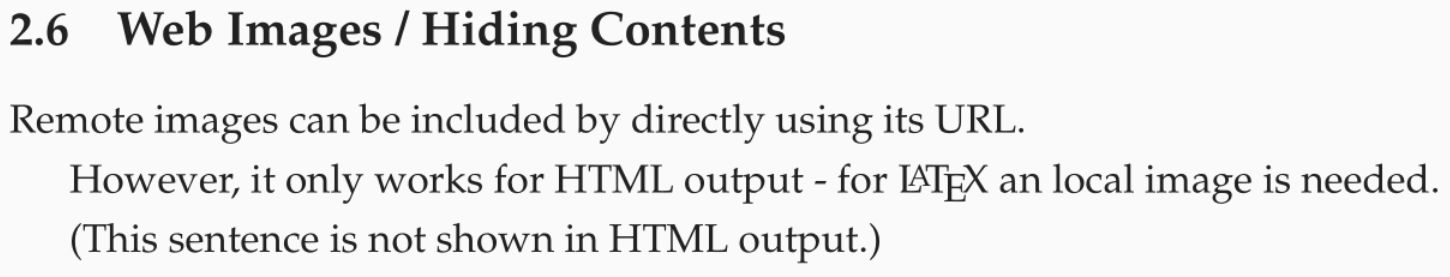
\includegraphics[width=7.5cm]{../../../Assets/Images/Org-Teaching/Quickstart_Lecture-Editing_Hiding-Contents-LaTeX.png}
\end{center}
\end{multicols}

\subsubsection{Make contents reusable}
\label{sec:org192744c}
One of the biggest advantage of using \texttt{Org-Coursepack} to prepare course
content is that users can put content in topic Org files, and include relevant
part in semester Org files as needed, leveraging Org mode's flexible inclusion
functionality. Putting contents on a central location and reusing them reduce
redundancy and managing them easier. For example, any improvements on content 
will be applied to all courses automatically, and users can put topic Org
files into version control and keep track of the improvements.

The following shows an example usage:

\begin{center}
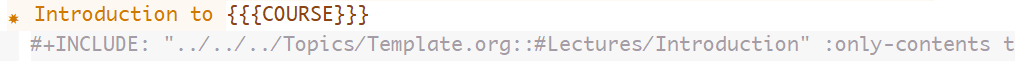
\includegraphics[height=0.8cm]{../../../Assets/Images/Org-Teaching/Quickstart_Lecture-Editing_Include.png}
\end{center}

Note that it is optional - users can put all course content to a semester Org
file directly. In fact, it is more convenient to do so when a course is
actively developed with new contents. We recommend, however, users to start
putting contents into relevant topic Org files as course content becomes more
stabilized. See \href{https://joonro.github.io/Org-Coursepack/Lectures/08\%2520Semester\%2520Org\%2520Files\%25203\%25204\%2520Lectures.html}{Lectures} part of the documentation for more information.
\subsection{Conclusion}
\label{sec:org4a34d0d}
That is it! The slide deck and the handout generated with the above examples can be 
\section{Overview of the Directory Structure}
\label{sec:org0c82b3d}
We present the directory structure of Org-Coursepack.

\begin{description}
\item[{\textbf{/Assets}}] This folder contains:
\begin{itemize}
\item Org setup files, which include frequently used macros (e.g., for LaTex
formatting).
\item Supplementary course materials (if any), such as images, videos, or
articles, for storage and access.
\end{itemize}
\item[{\textbf{/Assets/Institutions}}] This folder contains an institution Org file that
includes institution-specific information (e.g., university policies);
may have multiple Org files if teaching across multiple institutions.

\item[{\textbf{/Courses}}] Each unique course will have a subdirectory under \texttt{Courses}. A
course is defined as a series of lectures occupying a given
adademic calendar unit referred to as a semester. Same courses
may be offered across multiple semesters. Note that a course
may also have multiple sections in the same semester; for
example, a Statistics 101 course may be offered to three
different sets of students per semester.
\item[{\textbf{/Courses/Course}}] This folder contains:

\begin{itemize}
\item A course Org file that includes permanent information about the course
that remains consistent across semesters (e.g., syllabus items such as
learning objectives, grading schemes).
\item A subfolder for each semester this course is taught.
\end{itemize}

\item[{\textbf{/Courses/Course/Semester}}] Each semester folder contains:
\begin{itemize}
\item A semester Org file that includes information about the course that varies
by semester (e.g., classroom location, course schedule, assignment due
dates). The semester Org file also pulls information from other Org files,
such as course, topic, and institution Org files, to complete the course
development for that semester. In other words, this is the master file
that compiles all course materials for exporting.
\item Subfolders are for exported course materials (if any) and are
divided by type; i.e., Assignments, Lectures, Exams, and Syllabus.
\end{itemize}
\item[{\textbf{/Topics}}] This folder contains a topic Org file for each topic; these
files are where course content (e.g., lecture slides and notes,
exam questions, assignment guidelines) about specific topics
are stored and accessed.
\end{description}
\subsection{Example}
\label{sec:org62a2eb9}
The following example is the directory structure of this course, Org-Coursepack, as well as the template.

{\footnotesize
\begin{verbatim}
\
|
+---Assets
|   |   setup_Macros.org
|   |
|   +---Institutions
|           JOSE.org
|           Template.org
|
+---Courses
|   +---Org-Coursepack
|   |   |   Org-Coursepack.org
|   |   |
|   |   +---2018 Fall
|   |       |   2018 Fall.org
|   |       |
|   |       +---Assignments
|   |       |   |   Assignment 1.pdf
|   |       |   |   Assignment 1.tex
|   |       |
|   |       +---Lectures
|   |       |   |   01 Introduction.pdf
|   |       |   |   01 Introduction.tex
|   |       |
|   |       +---Exams
|   |       |   |   Exam 1.pdf
|   |       |   |   Exam 1.tex
|   |       |
|   |       +---Syllabus
|               |   Syllabus (Section 1).pdf
|               |   Syllabus (Section 1).tex
|   |
|   +---Template
|       |   Template.org
|       |   
|       +---Semester
|           |   Semester.org
|           |   
|           +---Assignments
|           |   |   Assignment_1.pdf
|           |   |   Assignment_1.tex
|           |           
|           +---Exams
|           +---Lectures
|           |   |   01 Introduction.pdf
|           |   |   01 Introduction.tex
|           |   |   
|           |           
|           +---Syllabus
|               |   Syllabus (Section 1).pdf
|               |   Syllabus (Section 1).tex
|
+---Topics
    |   Org-Teaching.org

\end{verbatim}
}
\end{document}